\section{Computational Methods} \label{sec:compmethod}
\subsection{Organising the Data}
Simon's foam simulation data comes in the form of a csv (comma-seperated value) file. To extract usable information for the python script, pandas is used to sort the data into a readable dataframe. \textit{Sample of data... see Appendix A: Listing \ref{lst:datasample}}.\\

\begin{lstlisting}[language=Python, caption=Organising csv data file into a usable dataframe, label=pandas]
    df = pd.read_csv(
        DATA_FILE,
        comment="#",
        sep=r"\s+",
        header=None,
        names=["id", "x", "y", "area", "pressure", "Z"]
    )
\end{lstlisting}

Using a pandas dataframe allows easy sorting of the data from the python script. For example, when calculating log-returns, it is most efficient to sort by \textit{id} first, then \textit{timestep} to ensure correct ordering, and calculate the log-returns for that bubble as per the definition. Another example, when calculating the average area, we instead want to sort by timestep and use the \textit{area} column to average over all bubbles in that timestep.\\

\begin{figure}[H]
    \centering
    \begin{minipage}[H]{0.48\textwidth}
        One of the first problems encountered when analysing the path of the bubbles was the \textbf{periodic boundary condition}. Figure \ref{fig:path-unfixed} shows that the bubble paths that cross over the border jump across to the opposite side of the plot. This is how the data is presented in the text file.\\
        To account for these jumps, using the length of the simulation box as found in the data file, a displacement limit of half the box can be used to flag large jumps, characterise whether it is in the x or y and rescale the x or y jump by the length of the box. Doing this leads to the proper paths of the bubbles as seen in figure \ref{bubbleallpath}.
    \end{minipage}
    \hfill
    \begin{minipage}[H]{0.48\textwidth}
        \centering
        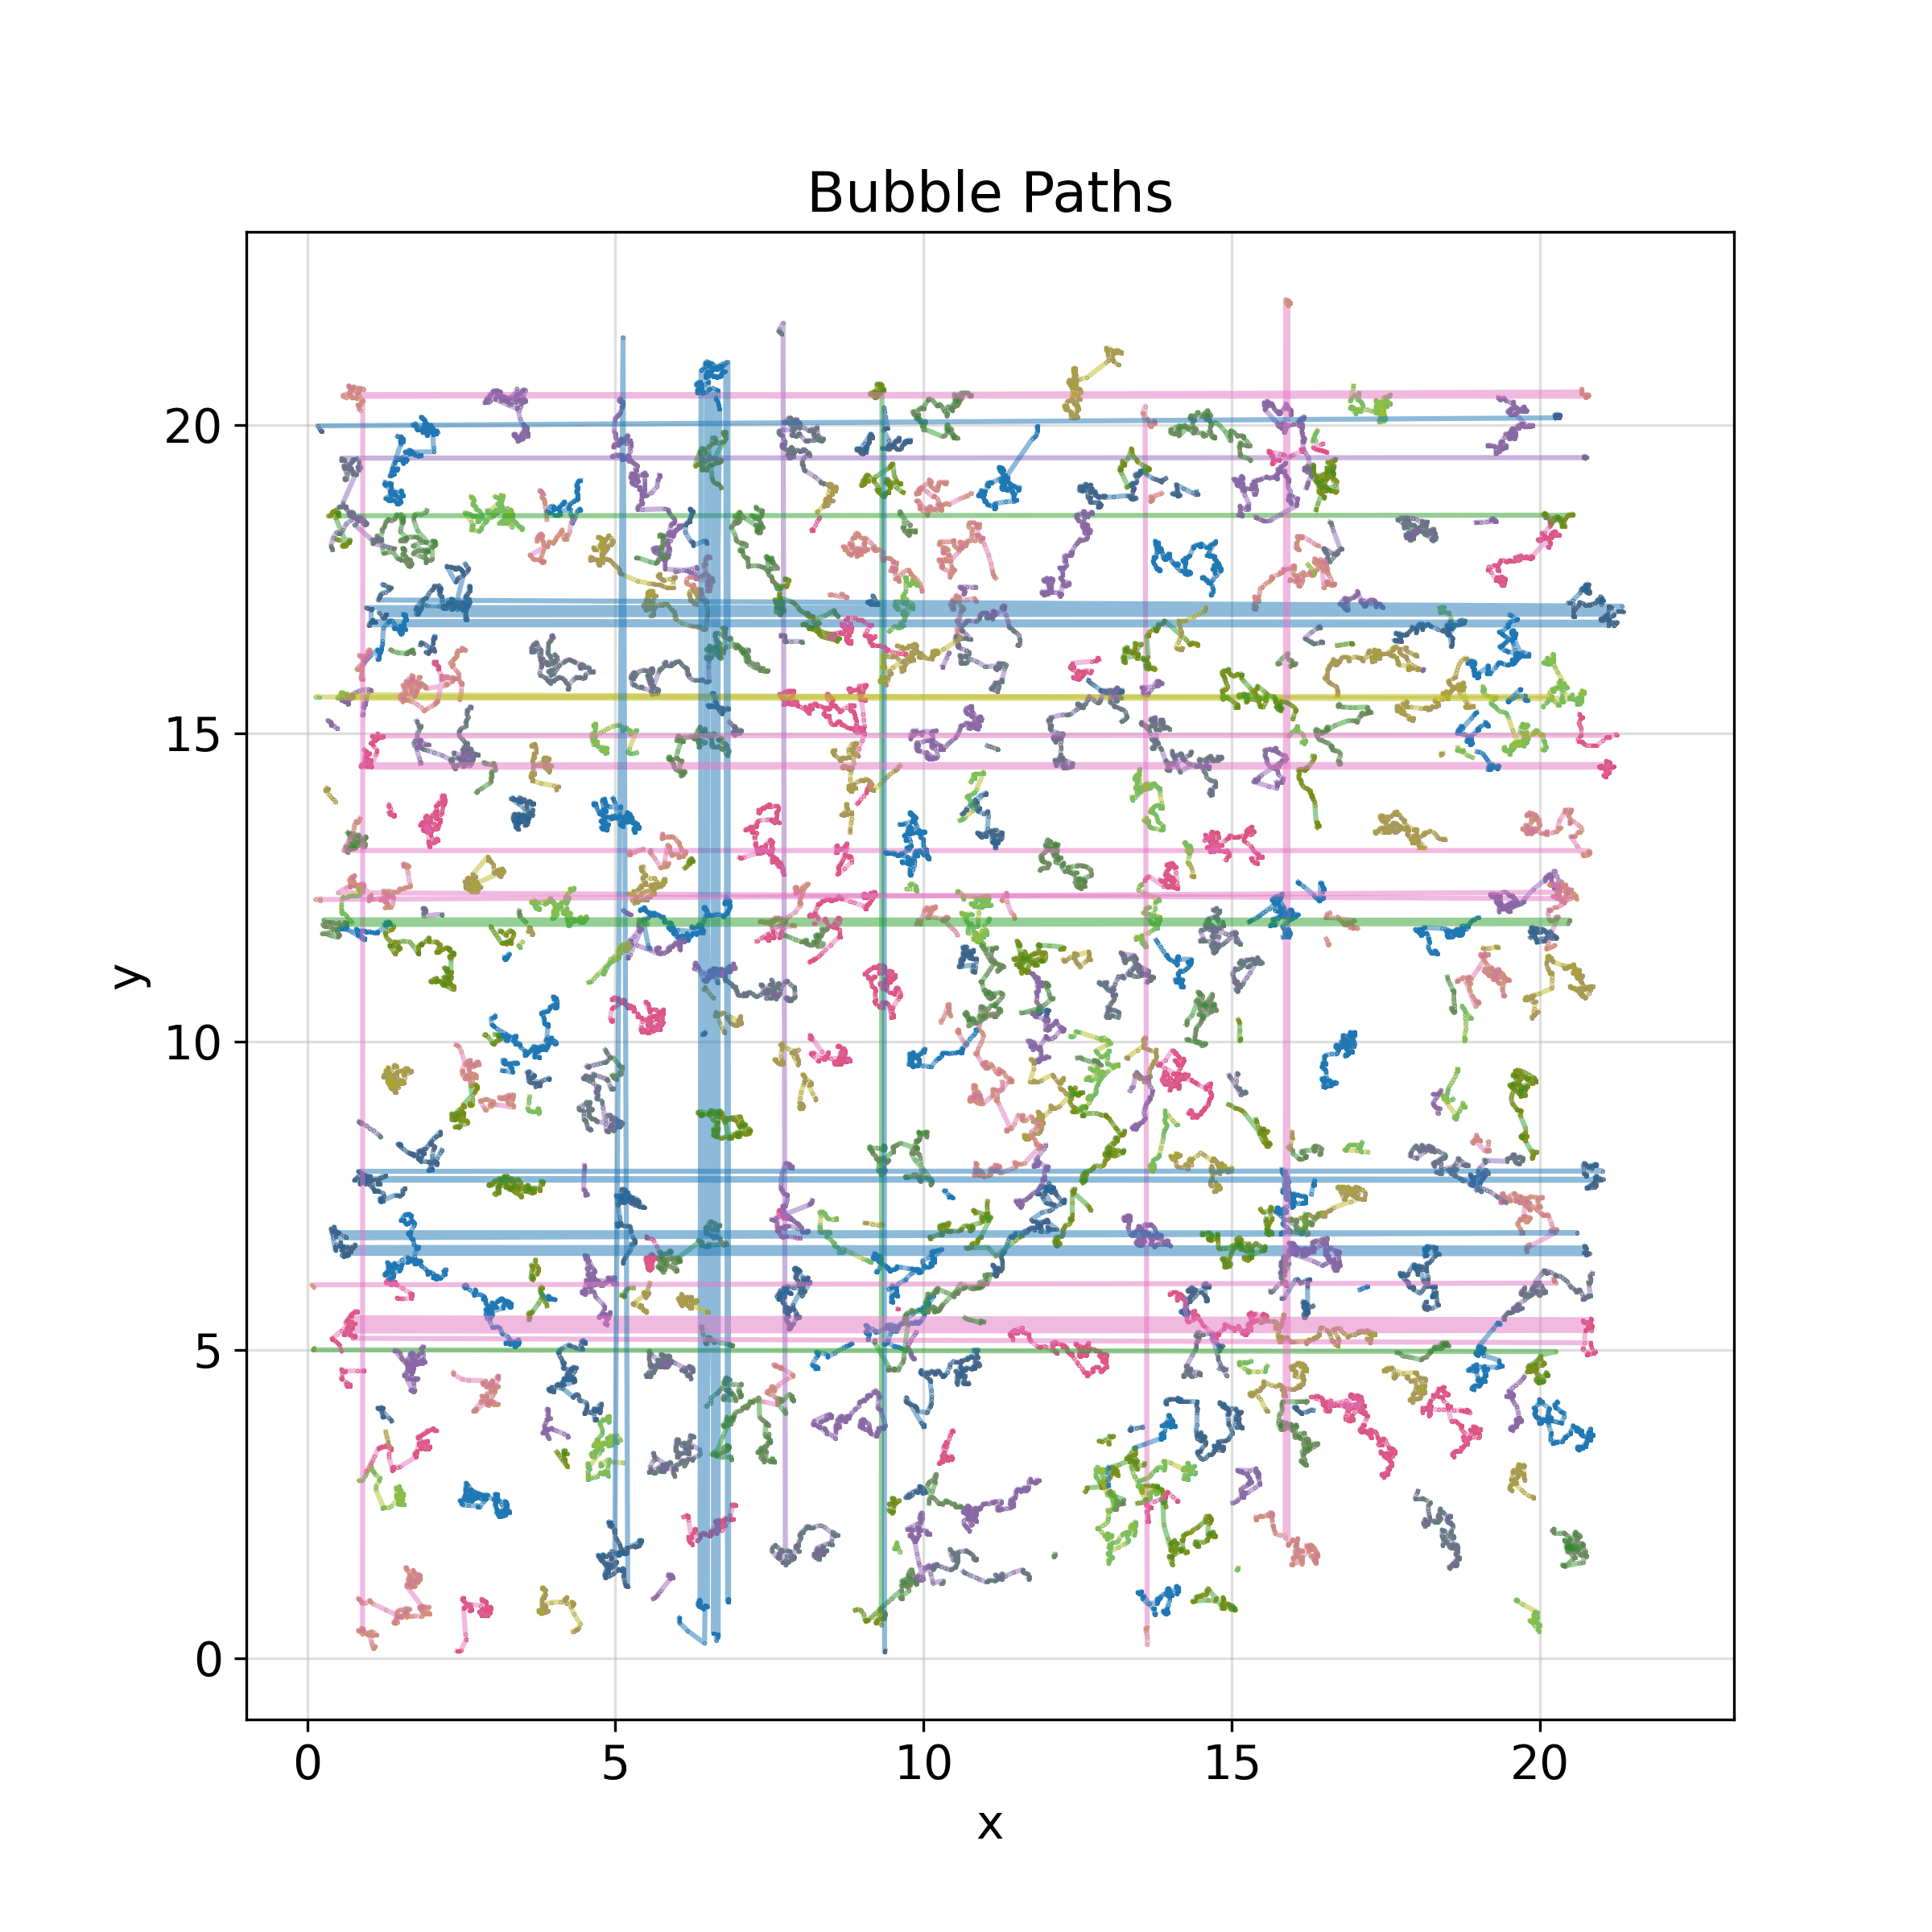
\includegraphics[width=\linewidth]{figures/bubble_paths_unfixed.png}
        \caption{Periodic boundary conditions need to be accounted for.}
        \label{fig:path-unfixed}
    \end{minipage}
\end{figure}

The best way found to do all this in conjunction with the analysis was to have a \code{data\_loader.py} file, where the data frame is made, the bubble paths are corrected and data files can be easily interchanged. All stored variables and data frames are then loaded into seperate Jupyter notebooks for each seperate statistical method to be applied and analysed.\\

\subsection{Brownian Motion}
In the interest of comparing directly with to the bubble motion, the Brownian walk parameters are chosen to match the dataset as closely as possible: 400 independent walks are made (equal the initial bubble count), each using 726 steps (equal the number of simulation timesteps), with step sizes taken from a zero-mean normal distribution. The choice of standard deviation is trivial as it is the shape of the statistics, displacement distributions, correlation functions, etc., that we are concerned with. For the MSD, the 2Dt relation can be plot on dimensionless axes to be independent on Brownian simulation parameters.\\

\subsection{Mean Squared Displacement}
To calculate the MSD, for each timestep, the squared displacement of each bubble (or Brownian step), $\delta r^2 = \delta x^2 + \delta y^2$, is calculated. As the name implies, the mean of the squared displacement is calculated and stored. Once this is done for all timesteps, the MSD can be plot versus time visualise the data.\\

An important difference when investigating the bubble MSD is that the number of bubbles is changing as seen in the survival curve, \textit{see Appendix B: \ref{fig:survcurv}}. Noting the milestones (300, 200, 100 bubbles for example), while plotting the MSD will be helpful in coming to a conclusions on how much of an effect the sample size has on the MSD relation, as seen in figure \ref{fig: MSD}.\\

\subsection{Log Returns}
Calculating the log returns is as simple as following the definition, equation \ref{eq:lr_def}, using x and y position as an analogue to the price $s(t)$. It is important to note that the radial position is used $r(t) = \sqrt{x(t)^2 + y(t)^2}$ since it is easier to analyse the autocorrelation function later, given concatenating the x log returns and y log returns (or displacements for that matter) wouldn't make physical sense for the ACF and volatility as they have temporal dependence (as oppose to a distribution where it is the magnitude of interest).\\

\subsection{Displacement Distribution}

\begin{figure}[H]
    \centering
    \begin{minipage}[H]{0.48\textwidth}
        The displacement distribution is trivially calcualted by looping over bubble id, sorting by timestep, and using the definition of displacement $\delta x(t, \Delta t) = x(t + \Delta t) - x(t)$ to calculate displacement in the x and y seperately. For the distributions, looking at figure \ref{fig:xycombine} it seems sufficient to concatenate the x and y displacements to get double the dataset and better overall statistics. However as mentioned in the previous section, the radial displacement will need to be taken into account instead when looking at the autocorrelation function. Varying $\Delta t$ can be done by looping over a list of $\Delta t$'s to analyse displacements over different time lags.
    \end{minipage}
    \hfill
    \begin{minipage}[H]{0.48\textwidth}
        \centering
        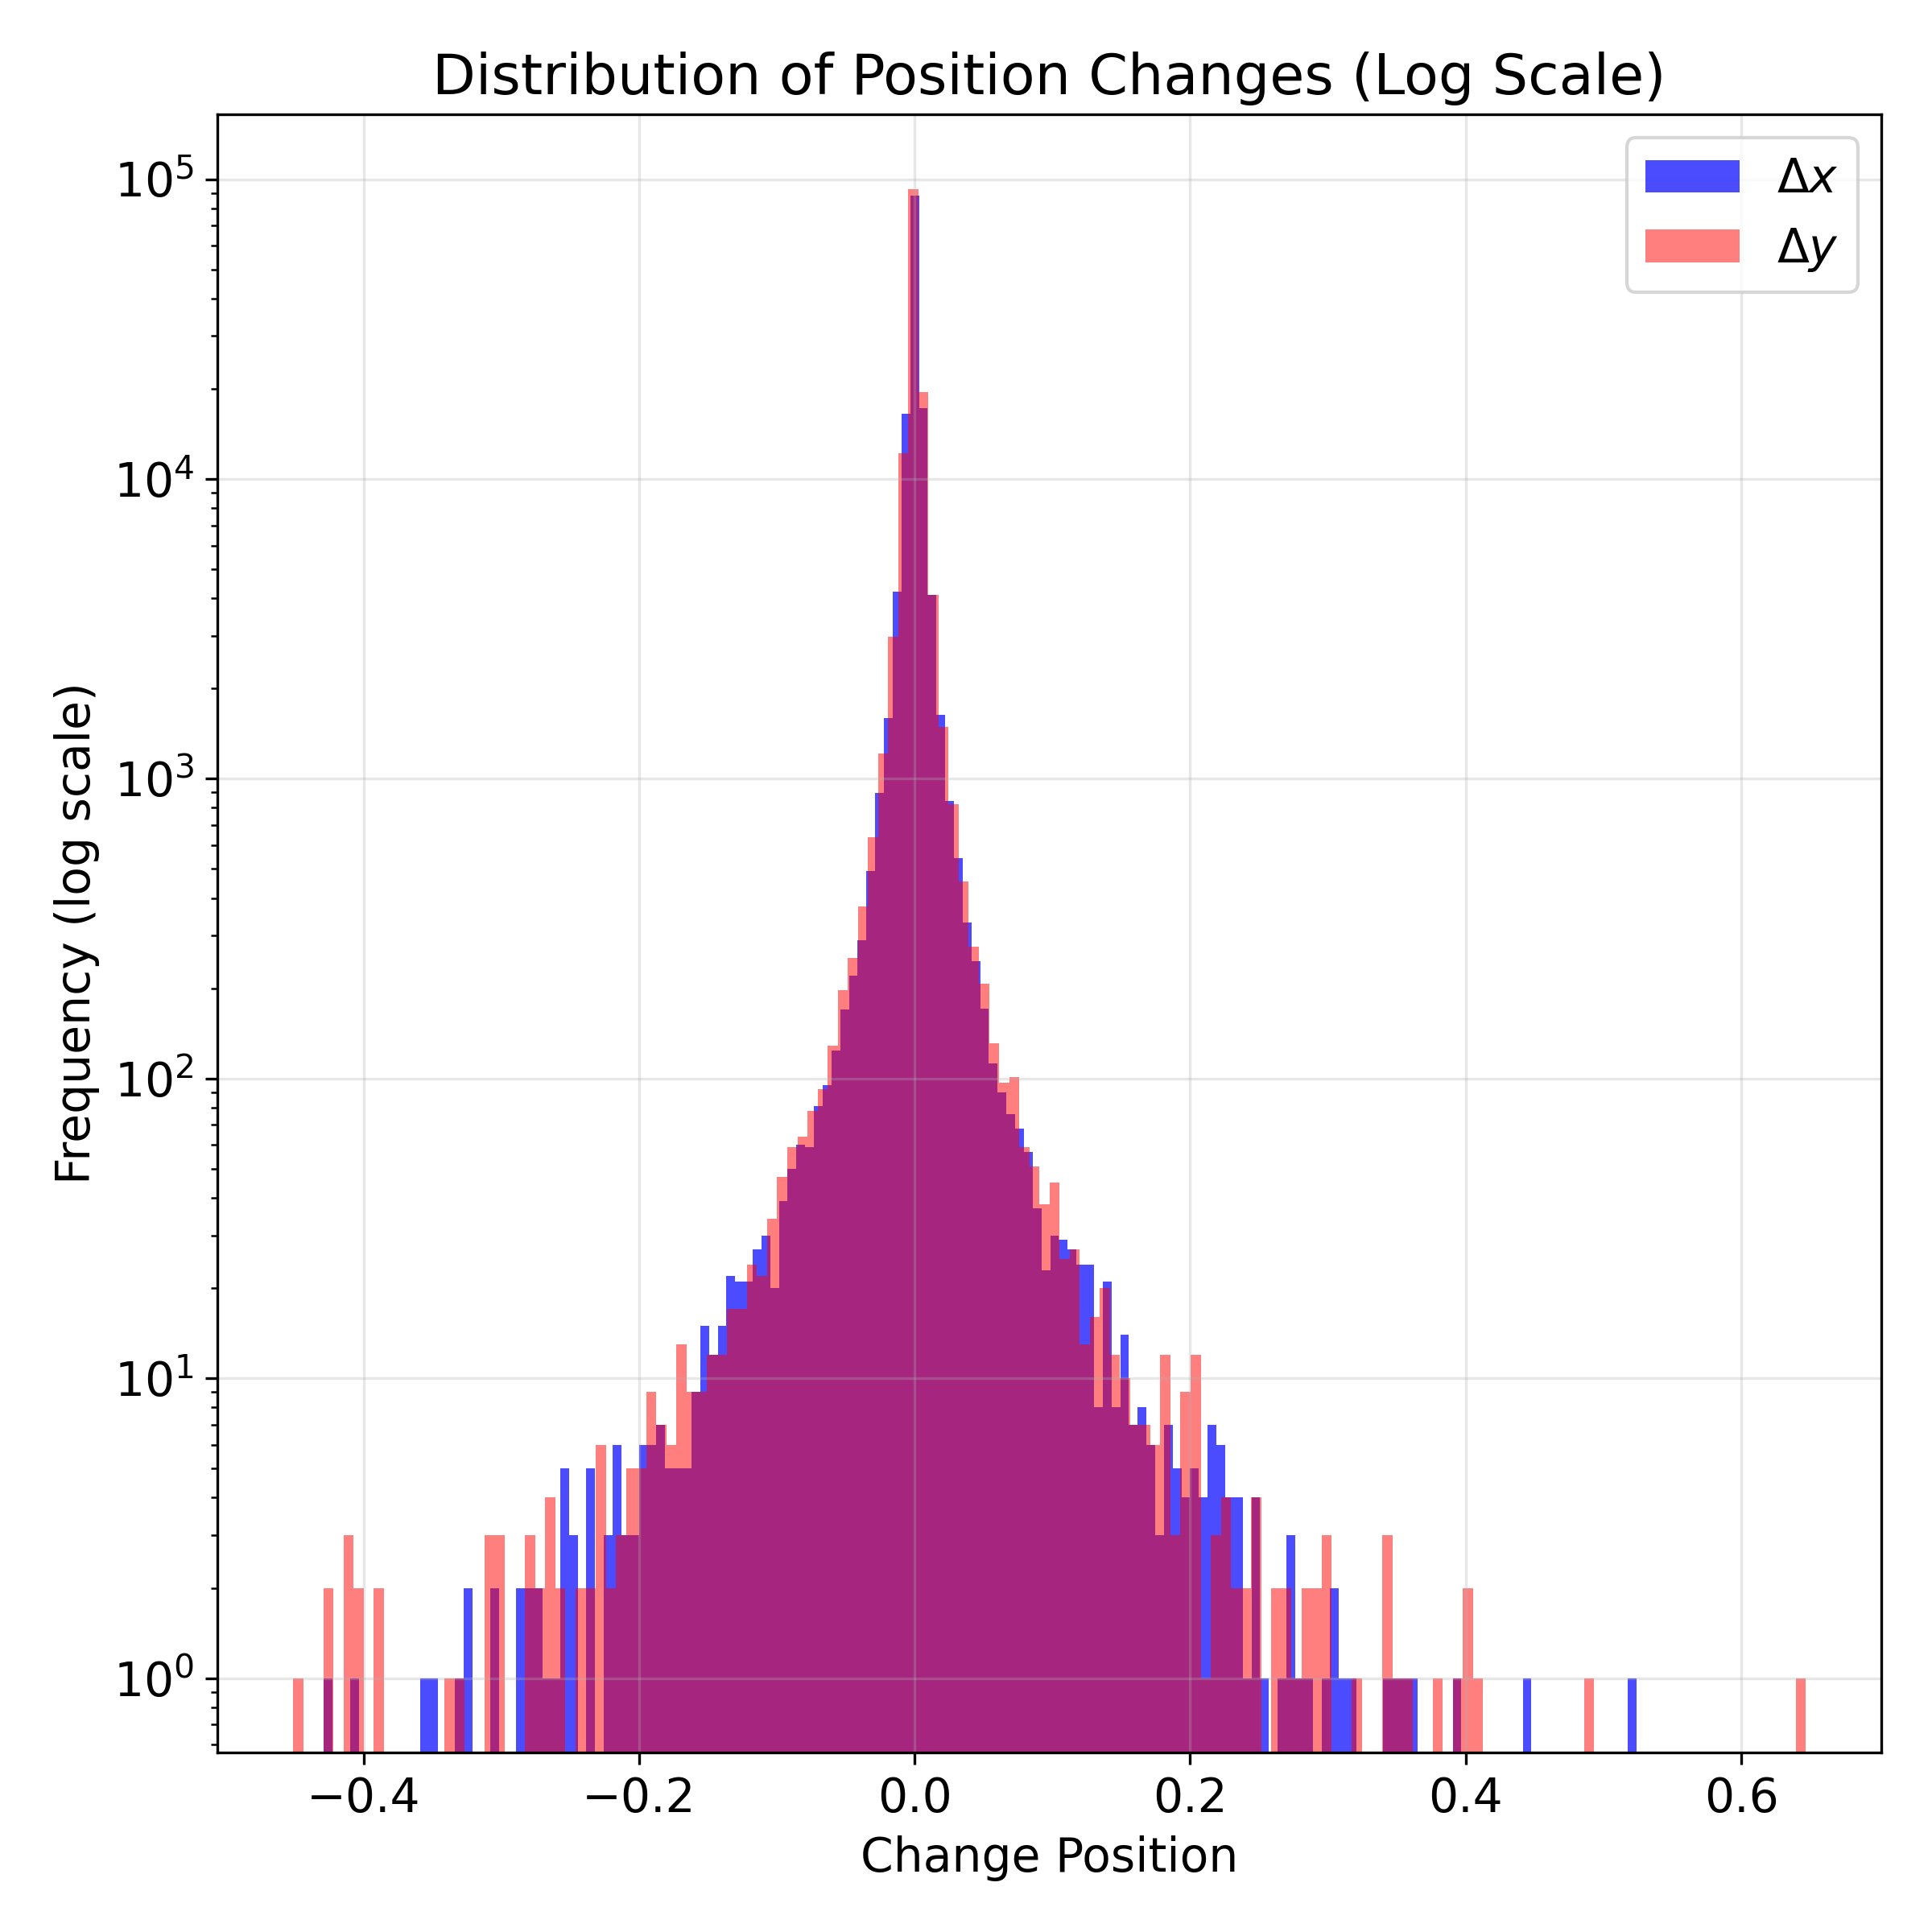
\includegraphics[width=\linewidth]{figures/x_y_combination_proof.png}
        \caption{x and y displacement distribution line up well enough to combine and get double the data.}
        \label{fig:xycombine}
    \end{minipage}
\end{figure}

\subsection{Complementary Cumulative Distribution Functions}
Using the CCDF to collapse the distributions onto a master plot consists of four main steps. The first, simply overlaying the displacement distributions on the one plot for varying $\Delta t$ and shifting the data for visual purposes so the distributions do not overlap. Second, using an integration method to obtain the CCDF itself. Third, taking probability cuts in the CCDFs (storing particular values in a list while calculating the CCDF) and plotting these values versus $\Delta t$ to get the scaling relation. Finally, using the slope of this CCDF scaling function to rescale the x axis of the original plot, using $x^\prime = x/\Delta t^\beta$ where $\beta$ is the slope, to collapse all distributions onto one master plot... in theory.\\


The numerical method used to find the CCDF is a sort-and-count method (\code{np.searchsorted}), which gives $P(|x|> X) = 1 - F(X)$ where $F(X)$ is the fraction of samples $\leq X$. This is a standard non-parametric Empirical Cumulative Distribution Function estimator, equivalent in principle to \code{matplotlib.axes.ecdf}, but evaluated 
over a uniform grid to allow direct comparison across $\Delta t$'s. This method is exact with respect to the sample does not introduce discretisation error unlike histogram-based approaches which require binning and therefore only approximate the ECDF \cite{MatplotlibECDF}. Methods such as Simpson's Rule are similarly unsuitable, as they require an estimation of the PDF, introducing approximation error before integration even begins.\\

If the slope $\beta$ is taken from figure \ref{fig:cutandcollapse_1}a, then $1/\beta$ is used as the Lévy parameter fitted to the peak of the distribution. When investigating the scaling properties of the CCDF further as seen in figure \ref{ccdfcutinvest}, the guess function (equation \ref{eq:scalefiteq}) is fit trivially via a least square fit to find the free parameters $c_1$ and $c_2$ associated with the fit.\\

\subsection{Temporal Autocorrelation Function}
As mentioned before, it is important to ensure the displacement and log returns in the x and y are calculated radially and not concatenated as there is a time dependence, and if the y data only kicks in halfway through the analysis of the ACF then we lose physical meaning.\\

In this project, the \textit{normalised autocorrelation function} is used, defined in section \ref{sec:temp_acf_def}. For each lag $\tau$, the ACF is computed directly as per it's definition equation \ref{eq:norm_acf}, \textit{as seen in Appendix A: Listing \ref{lst:acfcode}}.
